\chapter{Metrical TSP algorithms}


\section{Problem description}

\defproblem{ Metrical Travelling Salesman Problem}
{ Complete graph $G = (V,d)$, where $d:V \times V \to\mathbb{R}$ is a metric. }
{ What is the shortest cycle in $G$ which comes through every vertex exactly once? }

See link\footnote{\url{http://en.wikipedia.org/wiki/Travelling_salesman_problem}}
for detailed description.

\section{Christofides 1.5-apx}
Christofides algorithm\footnote{\url{http://en.wikipedia.org/wiki/Christofides_algorithm}} is designed to work with instances of TSP whose edge
weights satisfy triangle inequality. Let $G=(V, w)$ be an instance of TSP,
the algorithm consists of four steps:
\begin{enumerate}
\item Create minimum spanning tree $T$ for graph $G$. \\
Here we have implemented $\Oh(n^2)$ Prim's algorithm\footnote{\url{http://en.wikipedia.org/wiki/Prim's_algorithm}}.
Although for Euclidean spaces there exists faster $\Oh(n\log(n))$ algorithm, the overall gain
would be insignificant so we didn't use it.
\item Let $O$ be a set of odd degree vertices in $T$.
	  Find minimum perfect matching $M$ in complete graph over $O$. \\
For this part we have used \emph{Blossom V}\footnote{\url{http://pub.ist.ac.at/~vnk/software.html}}
implementation of Edmond's Blossom algorithm\footnote{\url{http://en.wikipedia.org/wiki/Blossom_algorithm}}.
Worst case running time of this part is $\Oh(|O|^5)$ but in average case it behaves very well.
\item Combine edges of $M$ and $T$ to form a multigraph $H$.
\item Find Eulerian circuit $E$ in $H$. ($\Oh(|H|)$).
\item Make $E$ Hamiltonian by shortcutting visited nodes. ($\Oh(|E|)$).
\end{enumerate}
Summing this up, our implementation in worst case needs $\Oh(|V|^5)$ time but generally
is fast in comparison to our other techniques.

\section{2opt Local Search}

In 2-opt\footnote{\url{http://en.wikipedia.org/wiki/2-opt}} local search for TSP, a single step
consists of reverting a segment of the current cycle. Intuitively, we find a point
at which the route crosses over itself and reorder it so that is doesn't.

Since in metrical TSP distance between a pair of points is the same for both directions,
computing fitness of the new route simplifies to removing a pair of edges and replacing it with another
pair.

We've tested 3 different structures for maintaining the current local search solution:
\begin{itemize}
\item array of vertices in order as they appear on the cycle.
\item Reversible Segment List\footnote{\url{http://www.hars.us/Papers/revi.pdf}}
\item Augmented splay tree.
\end{itemize}

\begin{tabular}{c|cc}
& vertex read cost & reverse cost \\\hline
array & $\Oh(1)$ & $\Oh(|V|)$ \\
RSL & $\Oh(\sqrt{|V|})$ & $\Oh(\sqrt{|V|})$ amortized \\
splay & $\Oh(\log(|V|)$ amortized & $\Oh(\log(|V|))$ amortized
\end{tabular}

In our implementation segment to reverse is selected with uniform probability,
excluding the degenerated cases -- set of cycle edges has to actually change.
Evaluating fitness of neighbouring solution drawn requires to read vertices
on 4 positions in the cycle. The number of fitness evaluations dominates
the number of the actual reverses in the long run due to the fact that it
becomes harder and harder to find a neighbour with better fitness as we approach
the local optimum. As a consequence we have empirically observed that out of
3 data structure mentioned, the array performed best on TSPLIB (see Benchmarks)
test cases.

\section{Monte Carlo Tree Search}
We will refer to the concepts and definitions introduced in MCTS design
chapter. Let us remind that the only domain-dependent concepts in our MCTS
framework are Move and State and the former is completely dependent on the
latter.

It is widely known from games solving applications of MCTS method that we
should choose State implementation which minimizes branch factor of resulting
search tree. For TSP problem we chose path building approach:
\begin{itemize}
  \item State is a path with arbitrary start point (permutation of a subset of
    all vertices)
  \item initial State is an arbitrary chosen start vertex
  \item Move represents choosing from remaining vertices the next one to be
    added to the end of the path
  \item terminal State is reached when all vertices are in the path
  \item Fitness of terminal State is equal to cost of a Hamilton cycle, note
    that path defines permutation of vertices and distance function is a proper
    metric
  \item Fitness estimate is a fitness of terminal state reached after applying
    a sequence of random decisions
\end{itemize}

We have introduced two improvements to above schema. In order to reduce branch
factor of resulting tree we have limited number of vertices taken into
consideration when choosing next move. A good heuristics here is to choose from
no more than $K$ vertices closest to the path's end.

To improve accuracy of each sample we have decided to replace last $L$ random
moves with exhaustive search, therefore Fitness estimate is set to minimum of
fitnesses of all terminal states visited during this search. Typically $N$ is
very small, for implementation described above we have determined that the best
accuracy to performance ratio can be achieved when $N = 4$, it should be
obvious that $N$ depends on the State implementation rather than size of the
input graph. Note that this method works well with certain types of policies
and statistics aggregation methods as discussed in results overview.

\section{Benchmarks}
To evaluate the algorithms quality we have used
TSPLIB\footnote{\url{http://comopt.ifi.uni-heidelberg.de/software/TSPLIB95/}}
symmetrical instances.

\section{Results}

We have selected the best local search algorithm to compare it against the best
MCTS and Christofides implementations on a subset of TSPLIB instances.
Additional experiments were performed to choose optimal configuration of a
local search and tree search algorithms, results of these tests are presented
later.

If $T$ is the running time of Christofides algorithm for given test instance
then the time limit for hill climb is set to $\max(T, 0.5 s)$ and for the tree
search is set to $\max(T, 5 s)$.

An $\infty$ in some cell means that no result could be obtained for given
instance using given algorithm within the time limit.

\begin{figure}[ht]
  \centering
  \begin{tabular}[ht]{|l||c|c|c|c|c|c|c|H}
\cline{1-8}
 & eil51 & eil76 & eil101 & pr152 & d198 & a280 & brd14051 & \\ \cline{1-8}\cline{1-8} 
Optimal &426 & 538 & 629 & 73682 & 15780 & 2579 & 469385 & \\ \cline{1-8}
HillClimb &458 & 593 & 704 & 76615 & 16741 & 2898 & 538022 & \\ \cline{1-8}
MonteCarloSearch &482 & 643 & 821 & 182894 & 34157 & 15186 & inf & \\ \cline{1-8}
Christofides &482 & 557 & 698 & 77585 & 17021 & 2830 & 524586 & \\ \cline{1-8}
\end{tabular}
\end{figure}

MCTS algorithm for TSP performed poorly when compared to other implemented
methods. Extensive comparison was unfortunately impossible due to extremely
high computational cost of the tree search method for instances with
significant number of vertices. Most of performed experiments used the smallest
instances available in TSPLIB collection -- graphs with less than $300$
vertices. The most efficient MCTS algorithm (see next section for model
selection methodology) needed at least $5 s$ to find a solution which was
$1.2$-approximation, while local search algorithms were able better solution
fraction of this time. Running the MCTS method for medium-sized instances is
impractical, for graphs with more than $10000$ vertices it is impossible.

Poor overall performance of MCTS method in our tests is a bit surprising as
travelling salesman problem variations are presented as a primary non-games
application of this approach (see \cite{MCTSsurvey} for details). We believe
that just like in the case of SA, the search space is too ,,smooth'' and
instead of making refined decisions one should check as many points as possible
within given time limit.

Our experiments showed that a simple hill climb local search heuristic performs
as well as Christofides algorithm. Given the complexity level of the latter
(finding a perfect matching with minimum weight) we can see no need to use
anything more complicated than a hill climb method for the symmetric metrical
TSP problem in practical applications.

\subsection { 2-opt hill climb \& simulated annealing }

In this experiment we've shown that SA doesn't improve the results of the 2-opt.
Initial temperature has been set to mean edge cost of the initial solution.
Temperature falls geometrically over time reaching fixed final temperature at the last iteration.
Diagrams 4.1-3 present SA with different final temperatures ($10^{-2}, 10^{-5}, 10^{-9}$) and
pure hill climb strategy on sample TSPLIB test cases.

\pgfsetplotmarksize{0pt}
\begin{figure}
 \centering
 \caption{\label{tsp_conv0}brazil58},
 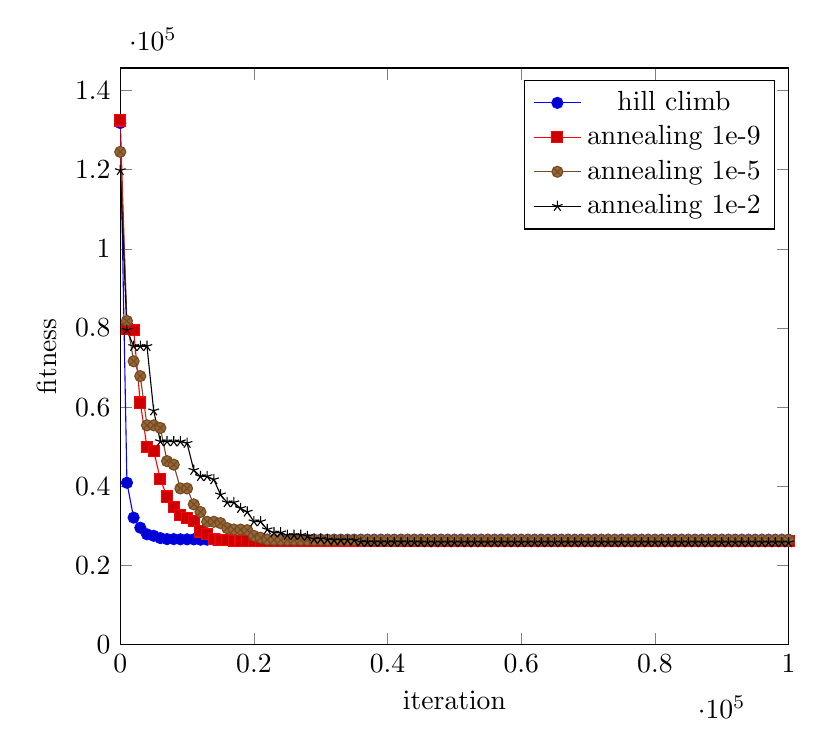
\begin{tikzpicture}
 \begin{axis}[
   width=0.7\textwidth,
   scale only axis,
   xlabel=iteration,
   ylabel=fitness,
   xmin=0,xmax=100000,ymin=0]
   \addplot coordinates {
     (0,131817)
     (1000,40879)
     (2000,32066)
     (3000,29518)
     (4000,27849)
     (5000,27470)
     (6000,26893)
     (7000,26633)
     (8000,26633)
     (9000,26590)
     (10000,26576)
     (11000,26576)
     (12000,26483)
     (13000,26483)
     (14000,26483)
     (15000,26483)
     (16000,26483)
     (17000,26483)
     (18000,26483)
     (19000,26483)
     (20000,26483)
     (21000,26483)
     (22000,26483)
     (23000,26483)
     (24000,26483)
     (25000,26483)
     (26000,26483)
     (27000,26483)
     (28000,26483)
     (29000,26483)
     (30000,26483)
     (31000,26483)
     (32000,26483)
     (33000,26483)
     (34000,26483)
     (35000,26483)
     (36000,26483)
     (37000,26483)
     (38000,26483)
     (39000,26483)
     (40000,26483)
     (41000,26483)
     (42000,26483)
     (43000,26483)
     (44000,26483)
     (45000,26483)
     (46000,26483)
     (47000,26483)
     (48000,26483)
     (49000,26483)
     (50000,26483)
     (51000,26483)
     (52000,26483)
     (53000,26483)
     (54000,26483)
     (55000,26483)
     (56000,26483)
     (57000,26483)
     (58000,26483)
     (59000,26483)
     (60000,26483)
     (61000,26483)
     (62000,26483)
     (63000,26483)
     (64000,26483)
     (65000,26483)
     (66000,26483)
     (67000,26483)
     (68000,26483)
     (69000,26483)
     (70000,26483)
     (71000,26483)
     (72000,26483)
     (73000,26483)
     (74000,26483)
     (75000,26483)
     (76000,26483)
     (77000,26483)
     (78000,26483)
     (79000,26483)
     (80000,26483)
     (81000,26483)
     (82000,26483)
     (83000,26483)
     (84000,26483)
     (85000,26483)
     (86000,26483)
     (87000,26483)
     (88000,26483)
     (89000,26483)
     (90000,26483)
     (91000,26483)
     (92000,26483)
     (93000,26483)
     (94000,26483)
     (95000,26483)
     (96000,26483)
     (97000,26483)
     (98000,26483)
     (99000,26483)
     (100000,26483)
   };
   \addlegendentry{hill climb}
   \addplot coordinates {
     (0,132467)
     (1000,79683)
     (2000,79453)
     (3000,61156)
     (4000,49924)
     (5000,48964)
     (6000,41805)
     (7000,37400)
     (8000,34659)
     (9000,32648)
     (10000,31995)
     (11000,31200)
     (12000,28565)
     (13000,27839)
     (14000,26586)
     (15000,26414)
     (16000,26414)
     (17000,26183)
     (18000,26175)
     (19000,26140)
     (20000,26133)
     (21000,26133)
     (22000,26133)
     (23000,26133)
     (24000,26133)
     (25000,26112)
     (26000,26112)
     (27000,26112)
     (28000,26112)
     (29000,26112)
     (30000,26112)
     (31000,26112)
     (32000,26112)
     (33000,26112)
     (34000,26112)
     (35000,26112)
     (36000,26112)
     (37000,26112)
     (38000,26112)
     (39000,26112)
     (40000,26112)
     (41000,26112)
     (42000,26112)
     (43000,26112)
     (44000,26112)
     (45000,26112)
     (46000,26112)
     (47000,26112)
     (48000,26112)
     (49000,26112)
     (50000,26112)
     (51000,26112)
     (52000,26112)
     (53000,26112)
     (54000,26112)
     (55000,26112)
     (56000,26112)
     (57000,26112)
     (58000,26112)
     (59000,26112)
     (60000,26112)
     (61000,26112)
     (62000,26112)
     (63000,26112)
     (64000,26112)
     (65000,26112)
     (66000,26112)
     (67000,26112)
     (68000,26112)
     (69000,26112)
     (70000,26112)
     (71000,26112)
     (72000,26112)
     (73000,26112)
     (74000,26112)
     (75000,26112)
     (76000,26112)
     (77000,26112)
     (78000,26112)
     (79000,26112)
     (80000,26112)
     (81000,26112)
     (82000,26112)
     (83000,26112)
     (84000,26112)
     (85000,26112)
     (86000,26112)
     (87000,26112)
     (88000,26112)
     (89000,26112)
     (90000,26112)
     (91000,26112)
     (92000,26112)
     (93000,26112)
     (94000,26112)
     (95000,26112)
     (96000,26112)
     (97000,26112)
     (98000,26112)
     (99000,26112)
     (100000,26112)
   };
   \addlegendentry{annealing 1e-9}
   \addplot coordinates {
     (0,124519)
     (1000,81784)
     (2000,71585)
     (3000,67836)
     (4000,55397)
     (5000,55397)
     (6000,54743)
     (7000,46341)
     (8000,45454)
     (9000,39448)
     (10000,39448)
     (11000,35419)
     (12000,33478)
     (13000,31016)
     (14000,31016)
     (15000,30678)
     (16000,29392)
     (17000,29048)
     (18000,29048)
     (19000,28905)
     (20000,27444)
     (21000,26973)
     (22000,26508)
     (23000,26450)
     (24000,26445)
     (25000,26433)
     (26000,26433)
     (27000,26433)
     (28000,26433)
     (29000,26433)
     (30000,26433)
     (31000,26433)
     (32000,26433)
     (33000,26433)
     (34000,26428)
     (35000,26428)
     (36000,26428)
     (37000,26428)
     (38000,26428)
     (39000,26428)
     (40000,26428)
     (41000,26428)
     (42000,26428)
     (43000,26428)
     (44000,26428)
     (45000,26428)
     (46000,26428)
     (47000,26428)
     (48000,26428)
     (49000,26428)
     (50000,26428)
     (51000,26428)
     (52000,26428)
     (53000,26428)
     (54000,26428)
     (55000,26428)
     (56000,26428)
     (57000,26428)
     (58000,26428)
     (59000,26428)
     (60000,26428)
     (61000,26428)
     (62000,26428)
     (63000,26428)
     (64000,26428)
     (65000,26428)
     (66000,26428)
     (67000,26428)
     (68000,26428)
     (69000,26428)
     (70000,26428)
     (71000,26428)
     (72000,26428)
     (73000,26428)
     (74000,26428)
     (75000,26428)
     (76000,26428)
     (77000,26428)
     (78000,26428)
     (79000,26428)
     (80000,26428)
     (81000,26428)
     (82000,26428)
     (83000,26428)
     (84000,26428)
     (85000,26428)
     (86000,26428)
     (87000,26428)
     (88000,26428)
     (89000,26428)
     (90000,26428)
     (91000,26428)
     (92000,26428)
     (93000,26428)
     (94000,26428)
     (95000,26428)
     (96000,26428)
     (97000,26428)
     (98000,26428)
     (99000,26428)
     (100000,26428)
   };
   \addlegendentry{annealing 1e-5}
   \addplot coordinates {
     (0,119830)
     (1000,79479)
     (2000,75385)
     (3000,75385)
     (4000,75385)
     (5000,59093)
     (6000,51315)
     (7000,51315)
     (8000,51281)
     (9000,51281)
     (10000,50895)
     (11000,44069)
     (12000,42484)
     (13000,42484)
     (14000,41698)
     (15000,37860)
     (16000,35884)
     (17000,35884)
     (18000,34417)
     (19000,33511)
     (20000,31073)
     (21000,31073)
     (22000,29056)
     (23000,28250)
     (24000,28250)
     (25000,27619)
     (26000,27619)
     (27000,27619)
     (28000,27336)
     (29000,26655)
     (30000,26655)
     (31000,26494)
     (32000,26319)
     (33000,26319)
     (34000,26319)
     (35000,26318)
     (36000,25886)
     (37000,25808)
     (38000,25808)
     (39000,25808)
     (40000,25808)
     (41000,25808)
     (42000,25808)
     (43000,25808)
     (44000,25808)
     (45000,25774)
     (46000,25766)
     (47000,25766)
     (48000,25766)
     (49000,25766)
     (50000,25761)
     (51000,25761)
     (52000,25761)
     (53000,25761)
     (54000,25761)
     (55000,25761)
     (56000,25761)
     (57000,25761)
     (58000,25761)
     (59000,25761)
     (60000,25761)
     (61000,25761)
     (62000,25761)
     (63000,25761)
     (64000,25761)
     (65000,25761)
     (66000,25761)
     (67000,25761)
     (68000,25761)
     (69000,25761)
     (70000,25761)
     (71000,25761)
     (72000,25761)
     (73000,25761)
     (74000,25761)
     (75000,25761)
     (76000,25761)
     (77000,25761)
     (78000,25761)
     (79000,25761)
     (80000,25761)
     (81000,25761)
     (82000,25761)
     (83000,25761)
     (84000,25761)
     (85000,25761)
     (86000,25761)
     (87000,25761)
     (88000,25761)
     (89000,25761)
     (90000,25761)
     (91000,25761)
     (92000,25761)
     (93000,25761)
     (94000,25761)
     (95000,25761)
     (96000,25761)
     (97000,25761)
     (98000,25761)
     (99000,25761)
     (100000,25761)
   };
   \addlegendentry{annealing 1e-2}
 \end{axis}
 \end{tikzpicture}
\end{figure}

\pgfsetplotmarksize{0pt}
\begin{figure}
 \centering
 \caption{\label{d15112}d15112},
 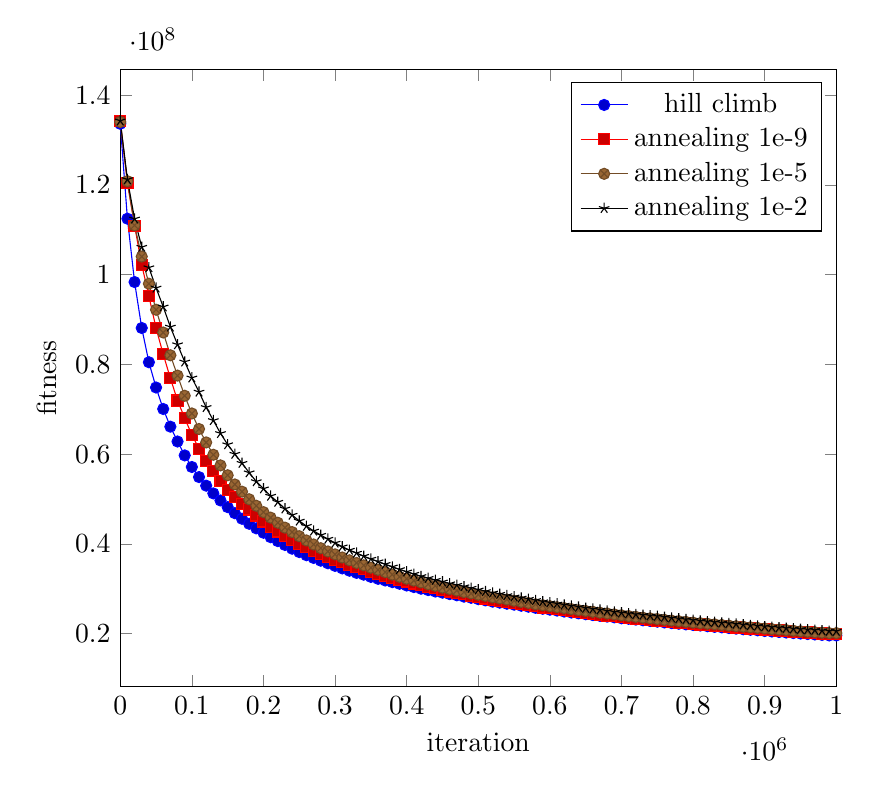
\begin{tikzpicture}
 \begin{axis}[
   width=0.75\textwidth,
   scale only axis,
   xlabel=iteration,
   ylabel=fitness,
   xmin=0,xmax=1000000]
   \addplot coordinates {
     (0,1.33636e+08)
     (10000,1.12488e+08)
     (20000,9.83696e+07)
     (30000,8.81319e+07)
     (40000,8.05017e+07)
     (50000,7.48699e+07)
     (60000,7.00832e+07)
     (70000,6.61463e+07)
     (80000,6.28384e+07)
     (90000,5.97424e+07)
     (100000,5.7159e+07)
     (110000,5.49105e+07)
     (120000,5.29947e+07)
     (130000,5.12696e+07)
     (140000,4.96985e+07)
     (150000,4.8218e+07)
     (160000,4.68654e+07)
     (170000,4.56269e+07)
     (180000,4.45044e+07)
     (190000,4.34847e+07)
     (200000,4.25034e+07)
     (210000,4.15186e+07)
     (220000,4.0646e+07)
     (230000,3.97839e+07)
     (240000,3.89547e+07)
     (250000,3.82003e+07)
     (260000,3.75036e+07)
     (270000,3.68946e+07)
     (280000,3.62796e+07)
     (290000,3.57045e+07)
     (300000,3.51211e+07)
     (310000,3.45634e+07)
     (320000,3.40531e+07)
     (330000,3.35632e+07)
     (340000,3.31642e+07)
     (350000,3.2669e+07)
     (360000,3.22379e+07)
     (370000,3.18679e+07)
     (380000,3.14996e+07)
     (390000,3.11325e+07)
     (400000,3.07518e+07)
     (410000,3.04045e+07)
     (420000,3.00349e+07)
     (430000,2.97272e+07)
     (440000,2.94108e+07)
     (450000,2.91538e+07)
     (460000,2.88339e+07)
     (470000,2.85738e+07)
     (480000,2.82688e+07)
     (490000,2.80133e+07)
     (500000,2.77073e+07)
     (510000,2.74378e+07)
     (520000,2.71536e+07)
     (530000,2.69292e+07)
     (540000,2.66875e+07)
     (550000,2.64853e+07)
     (560000,2.6243e+07)
     (570000,2.60287e+07)
     (580000,2.57743e+07)
     (590000,2.55723e+07)
     (600000,2.53639e+07)
     (610000,2.51671e+07)
     (620000,2.4942e+07)
     (630000,2.47267e+07)
     (640000,2.45422e+07)
     (650000,2.4352e+07)
     (660000,2.41537e+07)
     (670000,2.39813e+07)
     (680000,2.3826e+07)
     (690000,2.36513e+07)
     (700000,2.34505e+07)
     (710000,2.33306e+07)
     (720000,2.31572e+07)
     (730000,2.29973e+07)
     (740000,2.28515e+07)
     (750000,2.26934e+07)
     (760000,2.25218e+07)
     (770000,2.23746e+07)
     (780000,2.22357e+07)
     (790000,2.20895e+07)
     (800000,2.19558e+07)
     (810000,2.18392e+07)
     (820000,2.16797e+07)
     (830000,2.15317e+07)
     (840000,2.14297e+07)
     (850000,2.12759e+07)
     (860000,2.11426e+07)
     (870000,2.10028e+07)
     (880000,2.08838e+07)
     (890000,2.07661e+07)
     (900000,2.06157e+07)
     (910000,2.0496e+07)
     (920000,2.03848e+07)
     (930000,2.02735e+07)
     (940000,2.01563e+07)
     (950000,2.00486e+07)
     (960000,1.99411e+07)
     (970000,1.98414e+07)
     (980000,1.97386e+07)
     (990000,1.96267e+07)
     (1000000,1.96267e+07)
   };
   \addlegendentry{hill climb}
   \addplot coordinates {
     (0,1.34271e+08)
     (10000,1.20445e+08)
     (20000,1.10939e+08)
     (30000,1.02221e+08)
     (40000,9.52357e+07)
     (50000,8.80992e+07)
     (60000,8.22748e+07)
     (70000,7.69366e+07)
     (80000,7.19606e+07)
     (90000,6.80539e+07)
     (100000,6.43391e+07)
     (110000,6.12491e+07)
     (120000,5.84903e+07)
     (130000,5.62209e+07)
     (140000,5.40651e+07)
     (150000,5.20806e+07)
     (160000,5.0513e+07)
     (170000,4.89585e+07)
     (180000,4.7699e+07)
     (190000,4.63661e+07)
     (200000,4.50226e+07)
     (210000,4.38772e+07)
     (220000,4.27976e+07)
     (230000,4.18639e+07)
     (240000,4.09838e+07)
     (250000,4.00921e+07)
     (260000,3.92898e+07)
     (270000,3.85418e+07)
     (280000,3.78594e+07)
     (290000,3.7193e+07)
     (300000,3.65216e+07)
     (310000,3.59358e+07)
     (320000,3.5345e+07)
     (330000,3.48691e+07)
     (340000,3.43508e+07)
     (350000,3.38621e+07)
     (360000,3.3355e+07)
     (370000,3.29201e+07)
     (380000,3.25161e+07)
     (390000,3.20794e+07)
     (400000,3.16526e+07)
     (410000,3.12089e+07)
     (420000,3.08432e+07)
     (430000,3.04954e+07)
     (440000,3.0113e+07)
     (450000,2.9766e+07)
     (460000,2.94097e+07)
     (470000,2.91027e+07)
     (480000,2.87753e+07)
     (490000,2.84221e+07)
     (500000,2.81196e+07)
     (510000,2.78551e+07)
     (520000,2.76111e+07)
     (530000,2.72905e+07)
     (540000,2.70521e+07)
     (550000,2.68373e+07)
     (560000,2.66001e+07)
     (570000,2.63497e+07)
     (580000,2.60938e+07)
     (590000,2.58602e+07)
     (600000,2.56528e+07)
     (610000,2.54559e+07)
     (620000,2.52329e+07)
     (630000,2.5041e+07)
     (640000,2.47988e+07)
     (650000,2.46159e+07)
     (660000,2.4431e+07)
     (670000,2.42223e+07)
     (680000,2.40494e+07)
     (690000,2.38654e+07)
     (700000,2.3693e+07)
     (710000,2.35553e+07)
     (720000,2.33828e+07)
     (730000,2.31958e+07)
     (740000,2.30409e+07)
     (750000,2.29122e+07)
     (760000,2.27503e+07)
     (770000,2.259e+07)
     (780000,2.24605e+07)
     (790000,2.23235e+07)
     (800000,2.22104e+07)
     (810000,2.20718e+07)
     (820000,2.19426e+07)
     (830000,2.17856e+07)
     (840000,2.16615e+07)
     (850000,2.15245e+07)
     (860000,2.141e+07)
     (870000,2.12975e+07)
     (880000,2.11865e+07)
     (890000,2.10657e+07)
     (900000,2.09515e+07)
     (910000,2.08297e+07)
     (920000,2.07166e+07)
     (930000,2.05785e+07)
     (940000,2.0455e+07)
     (950000,2.0353e+07)
     (960000,2.026e+07)
     (970000,2.01533e+07)
     (980000,2.00475e+07)
     (990000,1.99308e+07)
     (1000000,1.99308e+07)
   };
   \addlegendentry{annealing 1e-9}
   \addplot coordinates {
     (0,1.3403e+08)
     (10000,1.20846e+08)
     (20000,1.10999e+08)
     (30000,1.04047e+08)
     (40000,9.80026e+07)
     (50000,9.21999e+07)
     (60000,8.71258e+07)
     (70000,8.20523e+07)
     (80000,7.75215e+07)
     (90000,7.30302e+07)
     (100000,6.90847e+07)
     (110000,6.56209e+07)
     (120000,6.26321e+07)
     (130000,5.98867e+07)
     (140000,5.75179e+07)
     (150000,5.5313e+07)
     (160000,5.32678e+07)
     (170000,5.1662e+07)
     (180000,4.99686e+07)
     (190000,4.8514e+07)
     (200000,4.70964e+07)
     (210000,4.5873e+07)
     (220000,4.4734e+07)
     (230000,4.36444e+07)
     (240000,4.26492e+07)
     (250000,4.17351e+07)
     (260000,4.07935e+07)
     (270000,3.98987e+07)
     (280000,3.90594e+07)
     (290000,3.83334e+07)
     (300000,3.76875e+07)
     (310000,3.6989e+07)
     (320000,3.63624e+07)
     (330000,3.57755e+07)
     (340000,3.52469e+07)
     (350000,3.47208e+07)
     (360000,3.4227e+07)
     (370000,3.37242e+07)
     (380000,3.31805e+07)
     (390000,3.2697e+07)
     (400000,3.22609e+07)
     (410000,3.18342e+07)
     (420000,3.1439e+07)
     (430000,3.10298e+07)
     (440000,3.06706e+07)
     (450000,3.02821e+07)
     (460000,2.99617e+07)
     (470000,2.9622e+07)
     (480000,2.928e+07)
     (490000,2.89886e+07)
     (500000,2.86968e+07)
     (510000,2.84342e+07)
     (520000,2.81109e+07)
     (530000,2.78748e+07)
     (540000,2.7632e+07)
     (550000,2.73449e+07)
     (560000,2.70867e+07)
     (570000,2.68538e+07)
     (580000,2.65635e+07)
     (590000,2.63519e+07)
     (600000,2.61346e+07)
     (610000,2.59222e+07)
     (620000,2.57152e+07)
     (630000,2.54845e+07)
     (640000,2.52494e+07)
     (650000,2.50818e+07)
     (660000,2.48922e+07)
     (670000,2.46873e+07)
     (680000,2.45198e+07)
     (690000,2.43134e+07)
     (700000,2.41107e+07)
     (710000,2.39412e+07)
     (720000,2.37732e+07)
     (730000,2.35847e+07)
     (740000,2.34313e+07)
     (750000,2.32651e+07)
     (760000,2.30958e+07)
     (770000,2.29271e+07)
     (780000,2.27983e+07)
     (790000,2.26506e+07)
     (800000,2.2495e+07)
     (810000,2.23592e+07)
     (820000,2.22377e+07)
     (830000,2.21064e+07)
     (840000,2.19568e+07)
     (850000,2.18246e+07)
     (860000,2.16893e+07)
     (870000,2.15709e+07)
     (880000,2.14308e+07)
     (890000,2.13043e+07)
     (900000,2.11825e+07)
     (910000,2.10325e+07)
     (920000,2.09213e+07)
     (930000,2.08182e+07)
     (940000,2.06786e+07)
     (950000,2.055e+07)
     (960000,2.04437e+07)
     (970000,2.03402e+07)
     (980000,2.02326e+07)
     (990000,2.01464e+07)
     (1000000,2.01464e+07)
   };
   \addlegendentry{annealing 1e-5}
   \addplot coordinates {
     (0,1.34312e+08)
     (10000,1.2123e+08)
     (20000,1.12453e+08)
     (30000,1.06158e+08)
     (40000,1.01601e+08)
     (50000,9.70668e+07)
     (60000,9.28618e+07)
     (70000,8.83708e+07)
     (80000,8.44418e+07)
     (90000,8.05924e+07)
     (100000,7.70358e+07)
     (110000,7.38771e+07)
     (120000,7.0456e+07)
     (130000,6.75427e+07)
     (140000,6.46617e+07)
     (150000,6.21554e+07)
     (160000,6.00351e+07)
     (170000,5.80075e+07)
     (180000,5.58993e+07)
     (190000,5.39322e+07)
     (200000,5.23234e+07)
     (210000,5.06913e+07)
     (220000,4.93444e+07)
     (230000,4.78523e+07)
     (240000,4.64543e+07)
     (250000,4.51423e+07)
     (260000,4.39858e+07)
     (270000,4.29114e+07)
     (280000,4.19779e+07)
     (290000,4.11072e+07)
     (300000,4.0233e+07)
     (310000,3.94036e+07)
     (320000,3.86516e+07)
     (330000,3.79932e+07)
     (340000,3.72947e+07)
     (350000,3.66535e+07)
     (360000,3.60851e+07)
     (370000,3.5491e+07)
     (380000,3.49178e+07)
     (390000,3.43376e+07)
     (400000,3.38113e+07)
     (410000,3.33008e+07)
     (420000,3.27887e+07)
     (430000,3.23735e+07)
     (440000,3.1948e+07)
     (450000,3.15867e+07)
     (460000,3.11723e+07)
     (470000,3.08497e+07)
     (480000,3.05151e+07)
     (490000,3.01796e+07)
     (500000,2.98042e+07)
     (510000,2.94404e+07)
     (520000,2.91124e+07)
     (530000,2.88311e+07)
     (540000,2.85302e+07)
     (550000,2.82428e+07)
     (560000,2.79951e+07)
     (570000,2.77168e+07)
     (580000,2.74523e+07)
     (590000,2.71646e+07)
     (600000,2.69117e+07)
     (610000,2.66779e+07)
     (620000,2.64148e+07)
     (630000,2.61934e+07)
     (640000,2.5957e+07)
     (650000,2.57205e+07)
     (660000,2.55242e+07)
     (670000,2.53269e+07)
     (680000,2.50635e+07)
     (690000,2.48576e+07)
     (700000,2.46707e+07)
     (710000,2.44964e+07)
     (720000,2.43175e+07)
     (730000,2.41625e+07)
     (740000,2.40235e+07)
     (750000,2.38965e+07)
     (760000,2.36986e+07)
     (770000,2.35386e+07)
     (780000,2.33602e+07)
     (790000,2.31765e+07)
     (800000,2.30209e+07)
     (810000,2.28547e+07)
     (820000,2.27108e+07)
     (830000,2.25777e+07)
     (840000,2.24329e+07)
     (850000,2.23029e+07)
     (860000,2.21652e+07)
     (870000,2.20065e+07)
     (880000,2.18576e+07)
     (890000,2.17405e+07)
     (900000,2.16061e+07)
     (910000,2.1473e+07)
     (920000,2.13518e+07)
     (930000,2.12347e+07)
     (940000,2.11202e+07)
     (950000,2.1003e+07)
     (960000,2.0912e+07)
     (970000,2.08105e+07)
     (980000,2.06966e+07)
     (990000,2.05899e+07)
     (1000000,2.05899e+07)
   };
   \addlegendentry{annealing 1e-2}
 \end{axis}
 \end{tikzpicture}
\end{figure}

\pgfsetplotmarksize{0pt}
\begin{figure}
 \centering
 \caption{\label{ulysses22}ulysses22},
 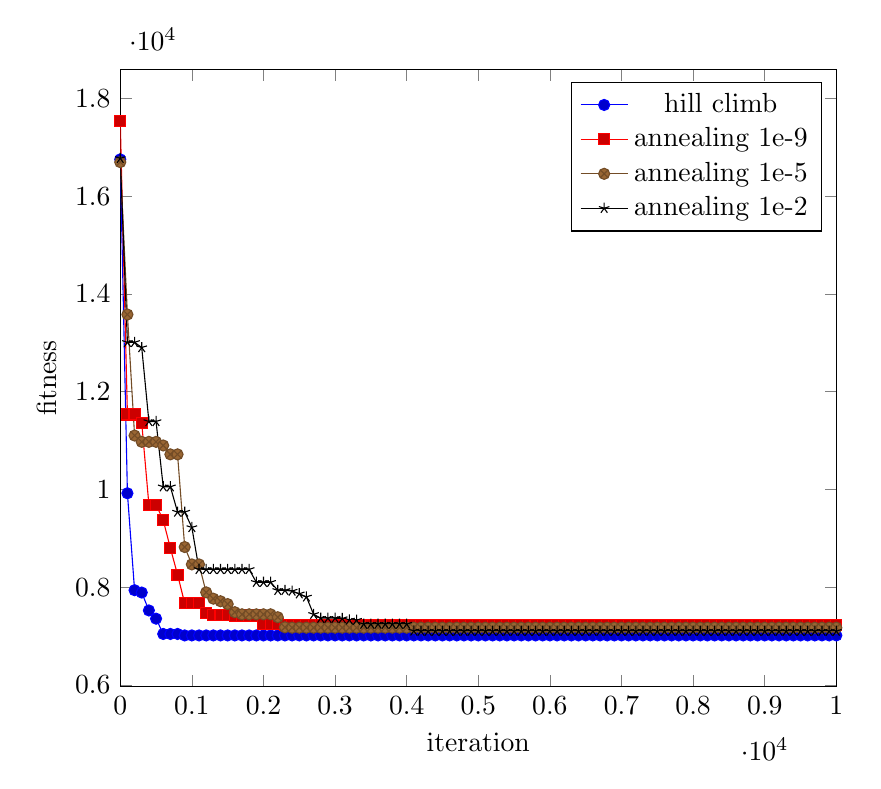
\begin{tikzpicture}
 \begin{axis}[
   width=0.75\textwidth,
   scale only axis,
   xlabel=iteration,
   ylabel=fitness,
   xmin=0,xmax=10000]
   \addplot coordinates {
     (0,16752)
     (100,9921)
     (200,7938)
     (300,7890)
     (400,7524)
     (500,7356)
     (600,7043)
     (700,7043)
     (800,7043)
     (900,7013)
     (1000,7013)
     (1100,7013)
     (1200,7013)
     (1300,7013)
     (1400,7013)
     (1500,7013)
     (1600,7013)
     (1700,7013)
     (1800,7013)
     (1900,7013)
     (2000,7013)
     (2100,7013)
     (2200,7013)
     (2300,7013)
     (2400,7013)
     (2500,7013)
     (2600,7013)
     (2700,7013)
     (2800,7013)
     (2900,7013)
     (3000,7013)
     (3100,7013)
     (3200,7013)
     (3300,7013)
     (3400,7013)
     (3500,7013)
     (3600,7013)
     (3700,7013)
     (3800,7013)
     (3900,7013)
     (4000,7013)
     (4100,7013)
     (4200,7013)
     (4300,7013)
     (4400,7013)
     (4500,7013)
     (4600,7013)
     (4700,7013)
     (4800,7013)
     (4900,7013)
     (5000,7013)
     (5100,7013)
     (5200,7013)
     (5300,7013)
     (5400,7013)
     (5500,7013)
     (5600,7013)
     (5700,7013)
     (5800,7013)
     (5900,7013)
     (6000,7013)
     (6100,7013)
     (6200,7013)
     (6300,7013)
     (6400,7013)
     (6500,7013)
     (6600,7013)
     (6700,7013)
     (6800,7013)
     (6900,7013)
     (7000,7013)
     (7100,7013)
     (7200,7013)
     (7300,7013)
     (7400,7013)
     (7500,7013)
     (7600,7013)
     (7700,7013)
     (7800,7013)
     (7900,7013)
     (8000,7013)
     (8100,7013)
     (8200,7013)
     (8300,7013)
     (8400,7013)
     (8500,7013)
     (8600,7013)
     (8700,7013)
     (8800,7013)
     (8900,7013)
     (9000,7013)
     (9100,7013)
     (9200,7013)
     (9300,7013)
     (9400,7013)
     (9500,7013)
     (9600,7013)
     (9700,7013)
     (9800,7013)
     (9900,7013)
     (10000,7013)
   };
   \addlegendentry{hill climb}
   \addplot coordinates {
     (0,17542)
     (100,11534)
     (200,11534)
     (300,11359)
     (400,9686)
     (500,9686)
     (600,9370)
     (700,8799)
     (800,8257)
     (900,7670)
     (1000,7670)
     (1100,7670)
     (1200,7479)
     (1300,7428)
     (1400,7428)
     (1500,7428)
     (1600,7420)
     (1700,7420)
     (1800,7420)
     (1900,7420)
     (2000,7246)
     (2100,7246)
     (2200,7246)
     (2300,7230)
     (2400,7230)
     (2500,7230)
     (2600,7230)
     (2700,7230)
     (2800,7230)
     (2900,7230)
     (3000,7230)
     (3100,7230)
     (3200,7230)
     (3300,7230)
     (3400,7230)
     (3500,7230)
     (3600,7230)
     (3700,7230)
     (3800,7230)
     (3900,7230)
     (4000,7230)
     (4100,7230)
     (4200,7230)
     (4300,7230)
     (4400,7230)
     (4500,7230)
     (4600,7230)
     (4700,7230)
     (4800,7230)
     (4900,7230)
     (5000,7230)
     (5100,7230)
     (5200,7230)
     (5300,7230)
     (5400,7230)
     (5500,7230)
     (5600,7230)
     (5700,7230)
     (5800,7230)
     (5900,7230)
     (6000,7230)
     (6100,7230)
     (6200,7230)
     (6300,7230)
     (6400,7230)
     (6500,7230)
     (6600,7230)
     (6700,7230)
     (6800,7230)
     (6900,7230)
     (7000,7230)
     (7100,7230)
     (7200,7230)
     (7300,7230)
     (7400,7230)
     (7500,7230)
     (7600,7230)
     (7700,7230)
     (7800,7230)
     (7900,7230)
     (8000,7230)
     (8100,7230)
     (8200,7230)
     (8300,7230)
     (8400,7230)
     (8500,7230)
     (8600,7230)
     (8700,7230)
     (8800,7230)
     (8900,7230)
     (9000,7230)
     (9100,7230)
     (9200,7230)
     (9300,7230)
     (9400,7230)
     (9500,7230)
     (9600,7230)
     (9700,7230)
     (9800,7230)
     (9900,7230)
     (10000,7230)
   };
   \addlegendentry{annealing 1e-9}
   \addplot coordinates {
     (0,16695)
     (100,13578)
     (200,11102)
     (300,10973)
     (400,10973)
     (500,10973)
     (600,10899)
     (700,10717)
     (800,10717)
     (900,8821)
     (1000,8466)
     (1100,8466)
     (1200,7894)
     (1300,7765)
     (1400,7712)
     (1500,7654)
     (1600,7488)
     (1700,7445)
     (1800,7445)
     (1900,7445)
     (2000,7445)
     (2100,7445)
     (2200,7385)
     (2300,7179)
     (2400,7172)
     (2500,7172)
     (2600,7172)
     (2700,7172)
     (2800,7172)
     (2900,7172)
     (3000,7172)
     (3100,7172)
     (3200,7172)
     (3300,7172)
     (3400,7172)
     (3500,7172)
     (3600,7172)
     (3700,7172)
     (3800,7172)
     (3900,7172)
     (4000,7172)
     (4100,7172)
     (4200,7172)
     (4300,7172)
     (4400,7172)
     (4500,7172)
     (4600,7172)
     (4700,7172)
     (4800,7172)
     (4900,7172)
     (5000,7172)
     (5100,7172)
     (5200,7172)
     (5300,7172)
     (5400,7172)
     (5500,7172)
     (5600,7172)
     (5700,7172)
     (5800,7172)
     (5900,7172)
     (6000,7172)
     (6100,7172)
     (6200,7172)
     (6300,7172)
     (6400,7172)
     (6500,7172)
     (6600,7172)
     (6700,7172)
     (6800,7172)
     (6900,7172)
     (7000,7172)
     (7100,7172)
     (7200,7172)
     (7300,7172)
     (7400,7172)
     (7500,7172)
     (7600,7172)
     (7700,7172)
     (7800,7172)
     (7900,7172)
     (8000,7172)
     (8100,7172)
     (8200,7172)
     (8300,7172)
     (8400,7172)
     (8500,7172)
     (8600,7172)
     (8700,7172)
     (8800,7172)
     (8900,7172)
     (9000,7172)
     (9100,7172)
     (9200,7172)
     (9300,7172)
     (9400,7172)
     (9500,7172)
     (9600,7172)
     (9700,7172)
     (9800,7172)
     (9900,7172)
     (10000,7172)
   };
   \addlegendentry{annealing 1e-5}
   \addplot coordinates {
     (0,16772)
     (100,13009)
     (200,13009)
     (300,12902)
     (400,11390)
     (500,11390)
     (600,10055)
     (700,10055)
     (800,9537)
     (900,9537)
     (1000,9222)
     (1100,8364)
     (1200,8364)
     (1300,8364)
     (1400,8364)
     (1500,8364)
     (1600,8364)
     (1700,8364)
     (1800,8364)
     (1900,8101)
     (2000,8101)
     (2100,8101)
     (2200,7935)
     (2300,7935)
     (2400,7921)
     (2500,7865)
     (2600,7801)
     (2700,7445)
     (2800,7366)
     (2900,7366)
     (3000,7366)
     (3100,7359)
     (3200,7330)
     (3300,7325)
     (3400,7244)
     (3500,7244)
     (3600,7244)
     (3700,7244)
     (3800,7244)
     (3900,7244)
     (4000,7244)
     (4100,7105)
     (4200,7100)
     (4300,7100)
     (4400,7100)
     (4500,7100)
     (4600,7100)
     (4700,7100)
     (4800,7100)
     (4900,7100)
     (5000,7100)
     (5100,7100)
     (5200,7100)
     (5300,7100)
     (5400,7100)
     (5500,7100)
     (5600,7100)
     (5700,7100)
     (5800,7100)
     (5900,7100)
     (6000,7100)
     (6100,7100)
     (6200,7100)
     (6300,7100)
     (6400,7100)
     (6500,7100)
     (6600,7100)
     (6700,7100)
     (6800,7100)
     (6900,7100)
     (7000,7100)
     (7100,7100)
     (7200,7100)
     (7300,7100)
     (7400,7100)
     (7500,7100)
     (7600,7100)
     (7700,7100)
     (7800,7100)
     (7900,7100)
     (8000,7100)
     (8100,7100)
     (8200,7100)
     (8300,7100)
     (8400,7100)
     (8500,7100)
     (8600,7100)
     (8700,7100)
     (8800,7100)
     (8900,7100)
     (9000,7100)
     (9100,7100)
     (9200,7100)
     (9300,7100)
     (9400,7100)
     (9500,7100)
     (9600,7100)
     (9700,7100)
     (9800,7100)
     (9900,7100)
     (10000,7100)
   };
   \addlegendentry{annealing 1e-2}
 \end{axis}
 \end{tikzpicture}
\end{figure}


The first problem which have been observed is that calculating temperature for boltzmann distribution is
expensive compared to a single iteration. We've dealt with it by updating temperature
only periodically. In our implementation mean SA iteration is about $30\%$ slower than
hill climb iteration. This fact hadn't been depicted on the diagrams in any way.

We can observe that hill climb converges strictly faster than any SA variant.
Moreover, the fitness curve is smooth (even though the neighbourhood is being browsed at random),
which means that not only 2-opt topology doesn't have many local optima but also that fitness function
is "continuous" in it.

Basing on these observations, we are not considering 2-opt SA a
suitable solution for TSP and have removed it from the general tsp comparison.

\subsection{Monte Carlo Tree Search policies}

Despite the poor performance of MCTS-based algorithms for TSP problem, we have
compared policies described in previous sections on small instances from
TSPLIB. The results are presented below. Each row corresponds to a single
policy (for names explanation please refer to the proper chapter). Each column
corresponds to the State representation being used. Column description has a
format \verb+<graph name>, limit <moves limit>+ where \emph{moves limit} is
the limit of the number of vertices taken into consideration when choosing next
move as described before. Number in each cell is equal to the final solution's
fitness.

The rest of configuration of each algorithm is exactly the same. In each test
run the algorithm preforms $500$ times the current number of vertices not in
the path samples per single decision.

\begin{figure}[ht]
  \centering
  \begin{tabular}[ht]{|l||c|c|c|c|H}
\cline{1-5}
 & eil51, limit 51 & eil51, limit 25 & eil51, limit 12 & eil51, limit 6 & \\ \cline{1-5}\cline{1-5} 
Optimal &426 & 426 & 426 & 426 & \\ \cline{1-5}
PolicyRandMean &480 & 464 & 480 & 522 & \\ \cline{1-5}
PolicyEpsMean &699 & 581 & 634 & 584 & \\ \cline{1-5}
PolicyEpsBest &992 & 996 & 859 & 650 & \\ \cline{1-5}
PolicyMuSigma &638 & 707 & 656 & 637 & \\ \cline{1-5}
\end{tabular}
\end{figure}

\begin{figure}[ht]
  \centering
  \begin{tabular}[ht]{|l||c|c|c|c|H}
\cline{1-5}
 & eil76, limit 76 & eil76, limit 38 & eil76, limit 19 & eil76, limit 9 & \\ \cline{1-5}\cline{1-5} 
Optimal &538 & 538 & 538 & 538 & \\ \cline{1-5}
PolicyRandMean &638 & 648 & 624 & 655 & \\ \cline{1-5}
PolicyEpsMean &1075 & 930 & 746 & 809 & \\ \cline{1-5}
PolicyEpsBest &1756 & 1567 & 1235 & 987 & \\ \cline{1-5}
PolicyMuSigma &950 & 930 & 1033 & 1005 & \\ \cline{1-5}
\end{tabular}
\end{figure}

\begin{figure}[ht]
  \centering
  \begin{tabular}[ht]{|l||c|c|c|c|H}
\cline{1-5}
 & eil101, limit 101 & eil101, limit 50 & eil101, limit 25 & eil101, limit 12 & \\ \cline{1-5}\cline{1-5} 
Optimal &629 & 629 & 629 & 629 & \\ \cline{1-5}
PolicyRandMean &742 & 754 & 811 & 757 & \\ \cline{1-5}
PolicyEpsMean &1364 & 1189 & 1081 & 1006 & \\ \cline{1-5}
PolicyEpsBest &2593 & 2118 & 1796 & 1408 & \\ \cline{1-5}
PolicyMuSigma &1262 & 1264 & 1277 & 1218 & \\ \cline{1-5}
\end{tabular}
\end{figure}

Results of this comparison were used while choosing the best algorithm's
configuration for other tests. We could also confirm a few observations made
during the course of fine-tunning our implementation.

Policies which choose the best node by minimizing expected fitness of a
solution outperform ones which minimize the lowest observed fitness and the
difference between them becomes smaller when the tree branch factor is being
reduced by restricting moves considered at each step. This can be heuristically
explained as a consequence of a performing exhaustive search when the size of
reachable solution's space is small enough (that means a few decisions before
reaching the terminal state). Once we are sure that after reaching a subtree
which is small enough we will find an optimal solution reachable from its root,
our objective is slightly different. Instead of looking for the best solution
we look for a subtree with pretty low fitness of reachable solutions in hope
that during the exhaustive search we will find better terminal state than we
have seen anytime before. We have made another observation which confirms above
conclusion. According to our tests the lowest fitness of any terminal state
reached during random sampling procedure is $5\% - 20\%$ higher than fitness of
the best state found during the final exhaustive search in the same run of an
algorithm.

Please note that the same pattern reproduces itself if one does not perform the
final exhaustive search. The main reason is that when the algorithm descends
into really small search subtree (say $6$ decisions before reaching the
terminal state) and the tree itself is highly uniform (estimates for each
children of a given node are roughly the same) all strategies reduce to picking
random path to some terminal state. When the number of samples per decision
exceeds the number of different terminal states the random sampling procedure
will visit all of them with high probability. The sole purpose of introduced
modification (the exhaustive search procedure) is to speed up entire process
and make sure that no matter how unlucky we are, we will always find the best
solution.

One can easily see that as far as the choice of the next node in the sampling
procedure is concerned there is no better strategy than uniform sampling. This
method is also the fastest one and its performance does not degrades when the
number of possible moves at each state (or a branch factor of the search tree)
increases. When one develops an algorithm which has a lot of magic constants
that affect its behaviour the problem of finding the best set of parameters
becomes nontrivial, uniform sampling is superior in this case as it guarantees
reasonable results without any fine tunning.

Note that the policies which prefer so-far-the best subtree during the random
sampling do not scale well when the branch factor of the search tree increases.
We suspect that these policies are completely useless for approximating
solution for instances with more than $100$ vertices as limiting the branch
factor greatly reduces reachable search space. Dramatically bad performance of
\emph{PolicyEpsBest} can be easily explained given the previous observations.
This policy not only seeks for a single best solution, which we already
investigated to be a bad idea, but also once a solution with low (but still far
from optimal) fitness is found in one subtree, the algorithm tends to visit
this subtree and greatly reduces chances of correcting this mistake.
